% !TEX root = Master.tex



As introduced in Section \ref{ssec:data_sources}, each article can be assigned to a set of attributes (see \autoref{tab:article_master_data}). 
%the setup of the data to be treated was introduced. As can be seen in \autoref{tab:article_master_data}, each article can be assigned to a set of attributes. 
Besides some elemental attributes like \textit{color}, \textit{age group} or \textit{gender}, the data exhibit a "natural" company-specific hierarchical structure. In \autoref{fig:article_hierarchy}, we can see an example of such a hierarchy for the attributes \textit{\ac{KCC}} and \textit{\ac{BS}} (see \autoref{tab:article_master_data}).
\\

\begin{figure}[H]
\centering
  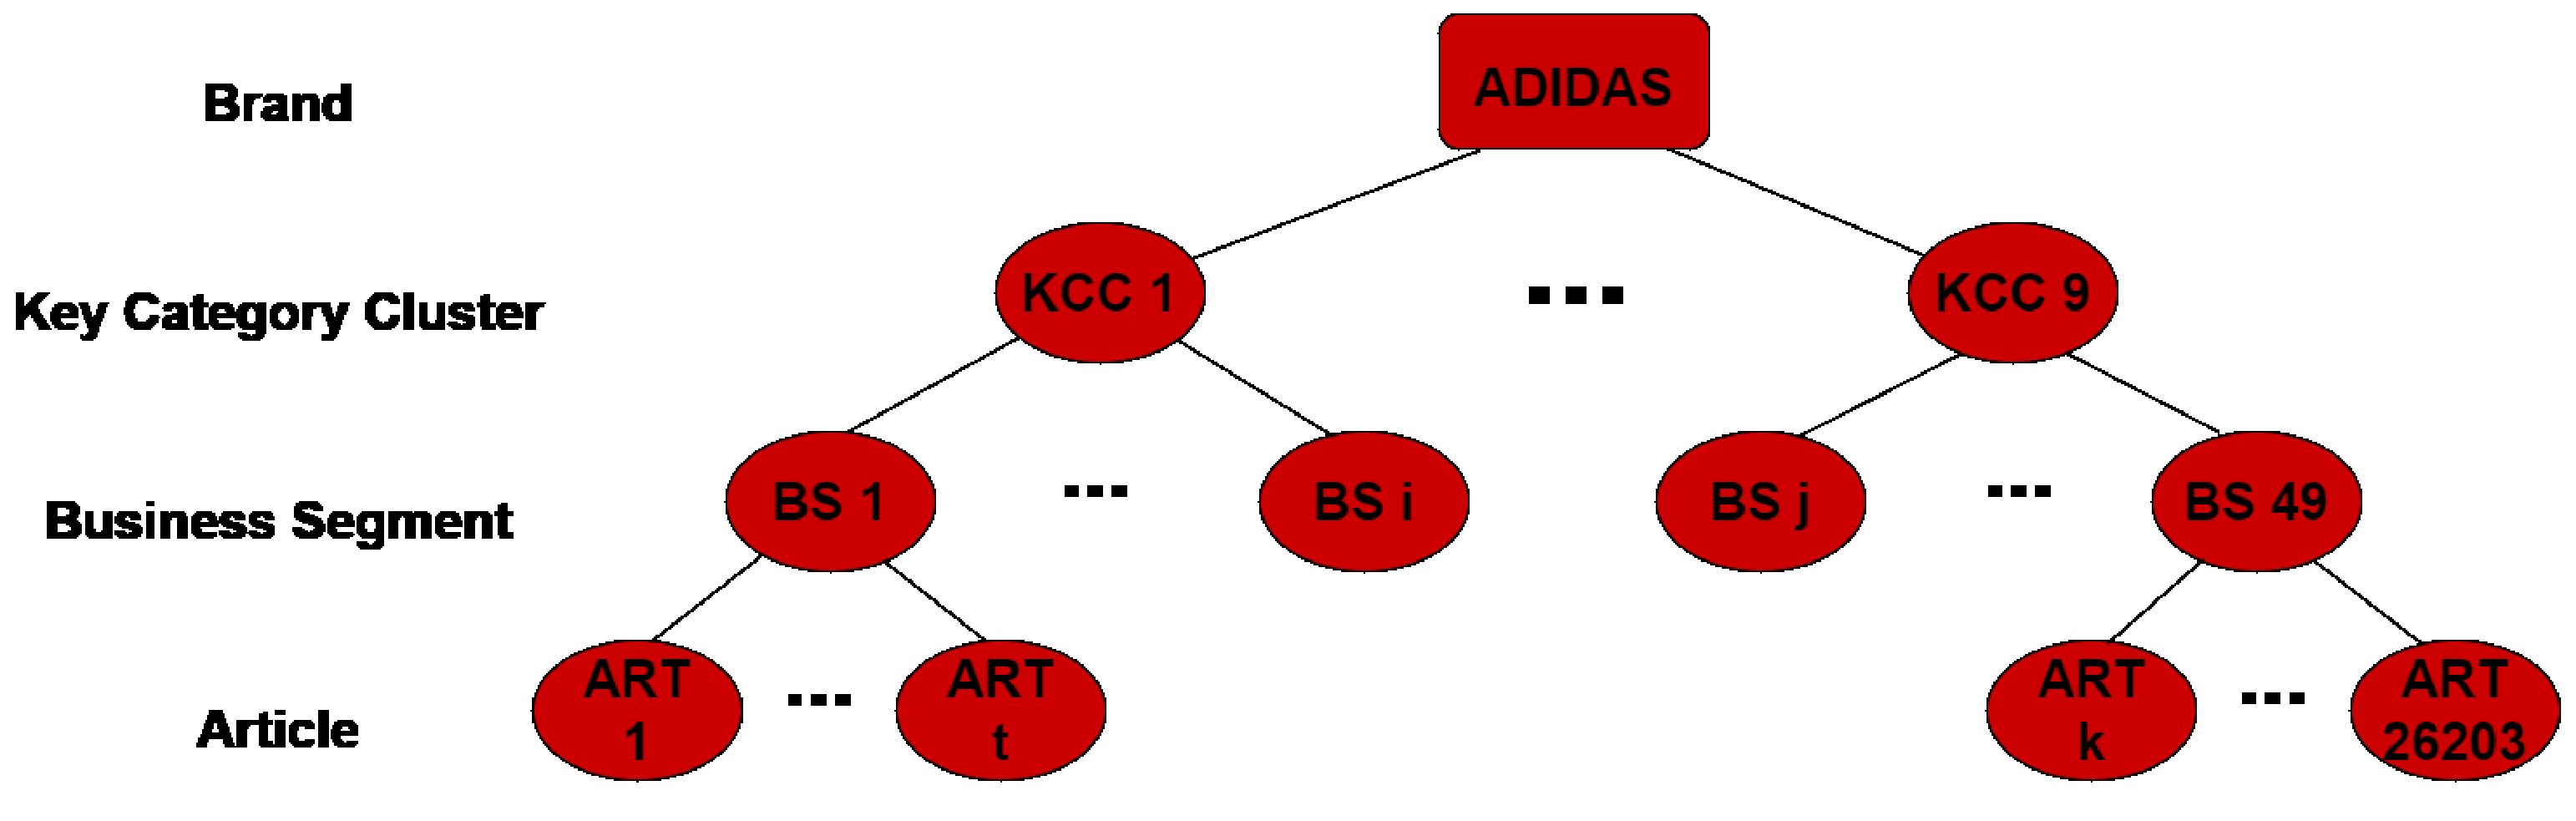
\includegraphics[width=0.95\linewidth]{figures/article_tree_KCC_BS.eps}
  \caption{Illustration of a hierarchical article structure}
  \label{fig:article_hierarchy}
\end{figure}

The bottom level consists of the individual articles and at the top level we have the brand. It is important to mention that there are more inner levels between the brand and the articles than depicted in \autoref{fig:article_hierarchy}. For example, \textit{\ac{KC}} would be the level below \textit{Key Category Cluster}. \textit{Key Category Clusters} are aggregated sport/fashion categories and \textit{Key Categories} add an additional layer to \textit{Key Category Clusters}, namely the \textit{Product Division} covering Footwear, Apparel and Accessories/Hardware. The \textit{Business Segment} supplements the \textit{Key Category} with a consumer driven "gender" perception.
Within the scope of this thesis, we are concerned with elements of the hierarchical structure depicted in \autoref{fig:article_hierarchy}, where for intermediate levels we focus on \textit{Key Category Cluster} only. In particular, our \textit{Key Category Clusters} of interest are \textit{"KCC 2"}, \textit{"KCC 6"} and \textit{"KCC 8"}.
\\
It is worth mentioning that some individual nodes might have only one single child node, meaning that the hierarchy level can stay consistent across multiple nodes. This phenomenon however is very rare and when it occurs, it affects usually two consecutive nodes. For instance, \textit{Sub-Brand 4} has only one child node \textit{KCC 6} (see \autoref{fig:single_childnode}).\footnote{Sub-Brands are visible for consumers through an own, not shared logo (see \autoref{fig:adidas_logos}).}
\\

\begin{figure}[H]
\centering
  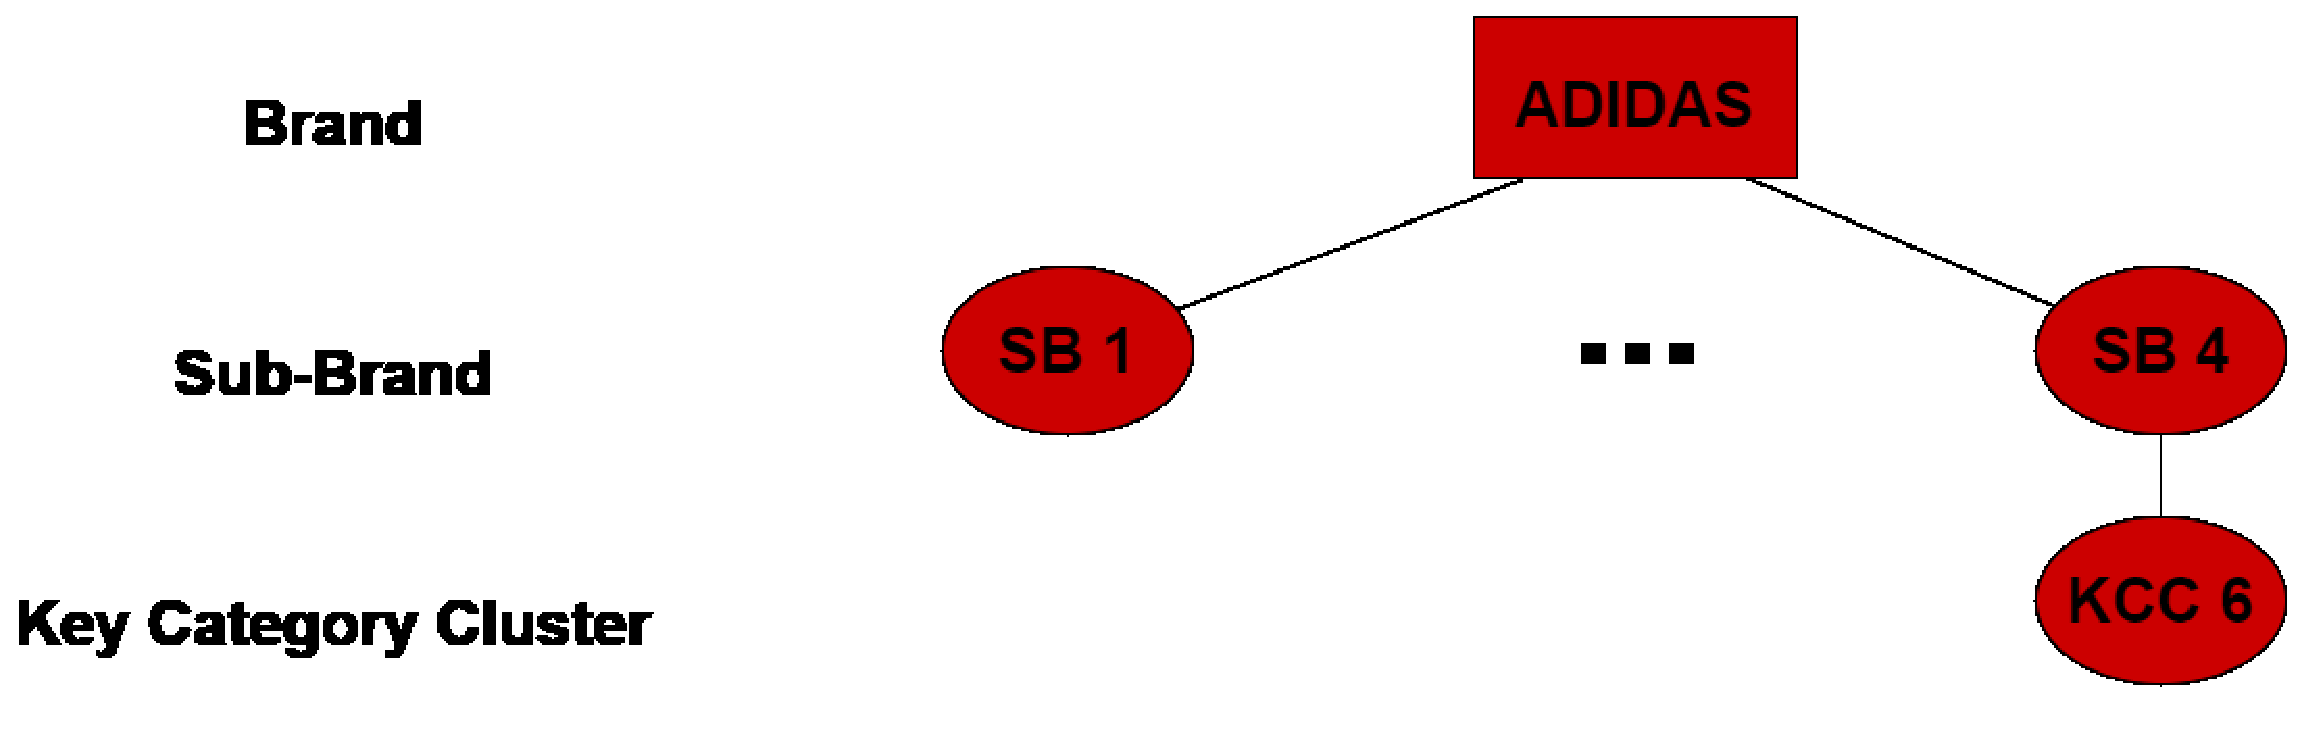
\includegraphics[width=.7\linewidth]{figures/article_tree_single_childnode.eps}
  \caption{Example of a single child node}
  \label{fig:single_childnode}
\end{figure} 










